\section{METODOLOGIA}

Este capítulo detalha os procedimentos metodológicos adotados para o diagnóstico e a mitigação da DT de documentação, bem como o contexto do sistema em que o estudo foi aplicado.

\subsection{Sistema de Fomento ao Microempreendedor}
\label{sec:sfm}

O SFM consiste em uma iniciativa do Governo do Estado da Paraíba, em parceria com o \textit{Artificial Intelligence Applications Laboratory} (ARIA) do Centro de Informática da Universidade Federal da Paraíba (CI/UFPB), voltada à criação de uma plataforma de contratação de serviços que, atualmente, encontra-se na fase de elaboração de seu Produto Mínimo Viável (MVP\footnote{O Produto Mínimo Viável (\textit{Minimum Viable Product}) consiste na versão mais elementar e funcional que um produto deve apresentar para validar hipóteses e entregar valor de negócio.}). Por intermédio desse sistema, servidores públicos registram as demandas de seus respectivos órgãos, o que habilita os prestadores vinculados à plataforma, a exemplo de Microempreendedores Individuais (MEIs), a submeterem propostas formais de execução. Desse modo, o ambiente virtual consolida-se como um canal de intermediação entre o ente contratante (órgão governamental) e o prestador contratado (MEI), o que viabiliza a seleção de profissionais e otimiza a divulgação das demandas da administração pública.

No escopo do sistema, as demandas de serviço registradas recebem a nomenclatura de ``oportunidades''. Uma vez cadastradas, tais oportunidades percorrem um fluxo operacional composto por sucessivas etapas: a aprovação prévia pelo gestor do órgão solicitante; a abertura do período para a submissão de propostas, que culmina na seleção da oferta mais vantajosa; a homologação dos resultados; a validação do contratado; a execução do serviço; e, por fim, o encerramento da oportunidade. Todas essas fases encontram-se mapeadas na plataforma com distintos graus de automação, destacando-se a etapa de seleção da proposta, a qual ocorre de maneira integralmente automatizada. Cabe ressaltar que, em estrita observância à Nova Lei de Licitações (Lei nº 14.133/2021) --- especificamente em seu Art. 95, § 2º, que regulamenta as pequenas compras e a prestação de serviços de pronto pagamento ---, apenas as demandas com custo estimado inferior ao teto legal (atualmente fixado na faixa de R\$ 13 mil) são elegíveis para registro no ambiente virtual.

Concluída a aprovação gerencial das oportunidades, inicia-se a fase de submissão de propostas. Durante esse período, os prestadores interessados elaboram ofertas nas quais especificam: o plano de execução do serviço; o prazo estimado para a sua conclusão; o orçamento total --- o qual engloba tanto os honorários quanto a eventual aquisição de materiais ---; e a documentação comprobatória de regularidade fiscal junto à Receita Federal. Esses dados são validados pela plataforma e, de modo subsequente, analisados pelos agentes públicos nas etapas de seleção e aprovação, respectivamente, configurando-se como requisitos obrigatórios em todas as submissões. Ademais, para cada oportunidade disponibilizada, o prestador de serviço restringe-se à vinculação de uma única proposta.

Embora a plataforma englobe outras funcionalidades e requisitos, a descrição supracitada delimita o escopo fundamental para a compreensão das análises conduzidas neste estudo. Ademais, regras de negócio e particularidades adicionais do sistema serão detalhadas nas seções subsequentes, à medida que se façam necessárias para a contextualização das discussões.

No que tange à dinâmica operacional, a equipe de desenvolvimento adotava práticas fundamentadas em metodologias ágeis. Nesse contexto, realizavam-se reuniões gerais semanais para a deliberação sobre as atividades concluídas e o planejamento das demandas subsequentes. Tais encontros resultavam na elaboração de atas de acompanhamento para o registro dessas tarefas. Em paralelo, as subequipes (\textit{design}, \textit{back-end}, \textit{front-end} e infraestrutura) conduziam alinhamentos periódicos próprios para o debate de pormenores de implementação, revisão de código (\textit{pull requests}) e resolução de impedimentos técnicos. Em linhas gerais, o regime de atuação ocorria em modalidade remota, envolvendo um contingente de aproximadamente 21 colaboradores --- em sua maioria discentes de graduação e pós-graduação ---, sob a coordenação de dois professores da própria UFPB. Por fim, sempre que a especificação de um novo requisito entrava em pauta, o fluxo de execução obedecia à seguinte estrutura:

\begin{enumerate}[topsep=0em, itemsep=0.3em]
   \item A nova funcionalidade era debatida de maneira concisa durante a reunião geral.
   \item Após a definição inicial do comportamento esperado, a equipe de \textit{design} elaborava os protótipos de interface correspondentes. A Figura~\ref{fig:tela_prototipo} ilustra uma das telas do sistema.
   \item A partir da disponibilização desses protótipos, as equipes de implementação iniciavam a codificação da funcionalidade, conforme a capacidade produtiva de cada frente de trabalho.
   \item Uma vez concluída a fase de implementação, a equipe de qualidade estruturava os casos de verificação fundamentando-se exclusivamente nas interfaces gráficas e em sua própria interpretação empírica sobre as regras de negócio implícitas.
\end{enumerate}

\begin{figure}[t]
    \centering
    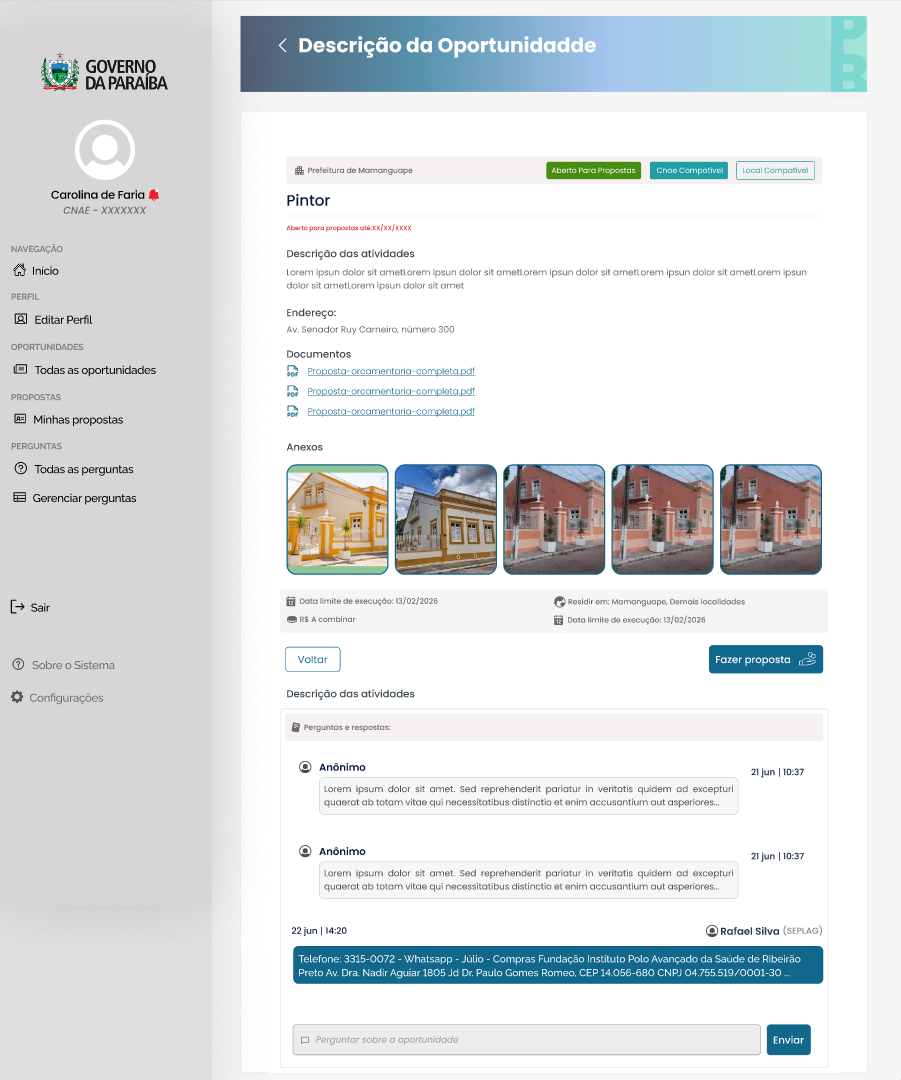
\includegraphics[height=15.8cm]{imagens/tela_prototipo.png}
    \caption{Protótipo da tela de visualização de oportunidades.}

    \vspace{3pt}
    {\small \textbf{Fonte:} Sistema de Fomento ao Microempreendedor.}
    
    \label{fig:tela_prototipo}
\end{figure}

\noindent Frequentemente, a etapa inicial desse fluxo era negligenciada ou conduzida de forma superficial, o que transferia para a equipe de \textit{design} a responsabilidade exclusiva de definição da lógica de operação das funcionalidades.

Complementarmente a esse fluxo, o projeto dispunha de um quadro \textit{Kanban} integrado ao repositório \textit{GitHub} para o rastreamento de tarefas (\textit{issues}). Tal ferramenta era empregada de maneira mais sistemática pelas equipes de infraestrutura e \textit{back-end}, bem como pelo time de Garantia de Qualidade (QA) para o registro de anomalias (\textit{bugs}). Cabe destacar, ainda, a divisão de responsabilidades nas rotinas de validação: a equipe de testes documentava os cenários acompanhados de suas respectivas massas de dados, focando estritamente em testes de sistema executados de forma manual, estruturados em formato tabular, conforme apresentado no Quadro~\ref{qua:exemplo_casos_teste}; em contrapartida, a elaboração dos testes de unidade e de integração constituía uma atribuição inerente aos próprios desenvolvedores.

A análise do fluxo de trabalho do projeto à luz da literatura sobre DT (ver Seção~\ref{sec:revisao_literatura}) revela que o SFM partilha de diversas vulnerabilidades estruturais recorrentes na indústria de \textit{software}. Observa-se que a negligência documental, motivada pela priorização de entregas em detrimento da especificação formal, instaura um cenário de falhas de comunicação e de ineficiência operacional. Embora a gestão de tarefas ocorra por meio de quadros \textit{Kanban} e de atas de reunião, a equipe carece de uma abordagem sistemática para o rastreamento das DTs, uma omissão comum em ambientes corporativos. Ademais, nota-se que o projeto contrai DTs de forma intencional mediante a elaboração acelerada de protótipos visuais. Ainda que essa tática seja válida para validar requisitos de alta incerteza, a ausência de um ``pagamento'' posterior --- consubstanciado na documentação formal das funcionalidades aprovadas --- converte essa estratégia em um gargalo de desenvolvimento. Por fim, a dependência exclusiva de rotinas de verificação inteiramente manuais agrava o ecossistema, impondo riscos de escalabilidade e de manutenibilidade que caracterizam os quadros severos de Dívida de Teste.

\begin{quadro}[t]
    \centering
    \caption{Exemplo do formato atual de documentação de casos de teste utilizado pela equipe de QA.}
    \label{qua:exemplo_casos_teste}
    
    \footnotesize
    % Aumentamos o respiro para 1.5, essencial para colunas com muito texto
    \renewcommand{\arraystretch}{1.5} 
    \renewcommand{\tabularxcolumn}[1]{m{#1}}
    
    % Adicionamos as barras verticais | para fechar as laterais e o miolo
    \begin{tabularx}{0.9\textwidth}{|>{\hsize=0.8\hsize}X|>{\hsize=1.2\hsize}X|>{\hsize=0.8\hsize}X|>{\hsize=1.2\hsize}X|c|}
        \hline
        \textbf{Caso de teste} & \textbf{Instruções} & \textbf{Dados} & \textbf{Resultados} & \textbf{Status} \\ 
        \hline % Substitui o midrule

        Login com credenciais válidas & 
        1. Abrir a tela de login \newline 2. Informar usuário válido \newline 3. Informar senha válida \newline 4. Clicar em ``Entrar'' & 
        \textbf{Usuário:} ******** \newline \textbf{Senha:} ******** & 
        \textbf{Esperado:} O sistema deve autenticar o usuário e redirecionar para a tela inicial. \newline \textbf{Obtido:} O sistema autenticou e redirecionou com sucesso. & Pass \\ 
        \hline % Adiciona separação entre as linhas de dados

        Login com apenas o usuário preenchido & 
        1. Abrir a tela de login \newline 2. Informar usuário válido \newline 3. Deixar senha vazia \newline 4. Clicar em ``Entrar'' & 
        \textbf{Usuário:} ******** \newline \textbf{Senha:} \newline(vazio) & 
        \textbf{Esperado:} Exibir mensagem de que a senha é obrigatória. \newline \textbf{Obtido:} Exibiu a mensagem corretamente. & Pass \\ 
        \hline % Substitui o bottomrule
    \end{tabularx}

    \vspace{5pt}
    \hspace*{0.25cm}\raggedright{\small \textbf{Fonte:} Sistema de Fomento ao Microempreendedor.}
\end{quadro}

\subsection{Delineamento do trabalho}

O presente trabalho caracteriza-se metodologicamente como um relato de experiên-\\cia fundamentado em um estudo de caso prático conduzido no escopo do SFM. Conforme embasado na revisão de literatura, a ausência ou a defasagem na especificação de requisitos configura uma DT que compromete severamente a garantia de qualidade de um \textit{software}. Com o intuito de mitigar o cenário diagnosticado no projeto e viabilizar a análise de completude dos casos de teste, determinou-se que a etapa precursora estritamente necessária seria a mapeação retrospectiva e a formalização dos requisitos. Ademais, buscou-se investigar a percepção da equipe técnica quanto ao andamento do desenvolvimento e ao impacto potencial da introdução desses artefatos formais em suas rotinas.


Para fins de clareza didática e estruturação lógica, a condução deste estudo dividiu-se em quatro fases principais: (i) delineamento e seleção da abordagem; (ii) procedimentos de mapeação e documentação; (iii) análise de rastreabilidade e cobertura; e (iv) levantamento e análise da percepção da equipe. Contudo, ressalta-se que, à semelhança das práticas ágeis da Engenharia de Software, os processos descritos a seguir não ocorreram de maneira estritamente linear, caracterizando-se por sobreposições e retroalimentações contínuas ao longo da execução do trabalho.

\subsection{Delineamento e seleção da abordagem}

Inicialmente, por meio da observação empírica e da condução de reuniões com os integrantes do projeto, mapeou-se a dinâmica operacional da equipe (conforme detalhado na Seção \ref{sec:sfm}). Constatou-se a adoção de um modelo de trabalho fundamentado em práticas ágeis, no qual a ênfase recaía sobre a interação do usuário com o sistema --- fato evidenciado pelo uso dos protótipos de interface como o principal artefato de documentação do projeto. Diante disso, estabeleceu-se que o método ideal para documentar os requisitos deveria preservar esse foco comportamental, mas, simultaneamente, suprir a carência técnica das equipes de implementação (\textit{back-end} e infraestrutura), as quais demandavam um detalhamento estrutural mais profundo sobre as respostas e lógicas internas do sistema. Sob essa ótica, a modelagem por Casos de Uso foi selecionada como a ferramenta de representação mais adequada.

A escolha pelos Casos de Uso em detrimento da adoção direta do BDD baseou-se em uma necessidade pragmática. Durante os alinhamentos, identificou-se que a simples escrita de cenários em linguagem natural não forneceria a granularidade técnica exigida pelos desenvolvedores. Contudo, visando facilitar uma futura transição da equipe para rotinas de automação de testes, os Casos de Uso foram estruturados com uma forte orientação comportamental, mantendo similaridade com a filosofia do BDD (ver Seção \ref{sec:engenharia_requisitos_teste_software}). Essa abordagem permitiu sanar a falta de detalhamento estrutural imediato, ao mesmo tempo em que manteve a especificação alinhada às práticas ágeis. Dessa forma, preparou-se o terreno não apenas para que a equipe de QA adote ferramentas como o Gherkin em trabalhos futuros, mas, sobretudo, para impulsionar a adoção de práticas formais e sistemáticas de documentação por todo o time de desenvolvimento.

\subsection{Procedimentos de mapeação e documentação}

Para a elaboração do documento, o contato direto com os stakeholders finais mostrou-se inviável, por se tratar de um projeto governamental sujeito a restrições de acesso. Diante desse cenário restritivo, a mapeação de requisitos e a identificação das regras de negócio ocorreram por meio de quatro frentes metodológicas: a análise de documentações legadas; o estudo dos protótipos de interface; a engenharia reversa do sistema em seu estado atual, conduzida sob a ótica de testes de caixa preta — isto é, mediante a exploração do software em funcionamento para o mapeamento empírico de seus comportamentos; e, sobretudo, a condução de reuniões de alinhamento com a equipe de desenvolvimento, abrangendo tanto os encontros gerais de planejamento quanto sessões técnicas pontuais. O conjunto de artefatos resultante desse levantamento foi redigido e versionado por intermédio da plataforma colaborativa \textit{Google Docs}.

Durante essa fase de coleta e especificação, constatou-se que a modelagem exclusiva por Casos de Uso seria insuficiente para representar a complexidade da plataforma. Essa limitação decorria das particularidades do domínio governamental e das restrições rigorosas sobre a estruturação e a exibição das informações transacionadas. Diante dessa necessidade, a documentação foi expandida para contemplar, além das interações, a formalização das RNs e a construção de Dicionários de Dados\footnote{Os dicionários de dados configuram-se como artefatos tabulares destinados a especificar as propriedades, os formatos e as restrições de tratamento aplicáveis a cada atributo manipulado pelo sistema.}. Por fim, em virtude da defasagem do acervo documental prévio, da inacessibilidade aos clientes e da priorização do alinhamento comportamental para o time de desenvolvimento, delimitou-se o escopo desta pesquisa estritamente aos requisitos funcionais, às RNs e aos dicionários de dados. O mapeamento dos requisitos não funcionais foi, portanto, elencado como perspectiva para trabalhos futuros (ver Seção~\ref{sec:conclusao}).

\subsection{Análise de rastreabilidade e cobertura}

Uma vez consolidada e aprovada por um dos coordenadores do projeto a primeira versão do novo documento formal de requisitos — concretizando, assim, a etapa basilar de especificação —, iniciou-se a fase de avaliação de completude. Para viabilizar esse processo, efetuou-se o mapeamento das relações entre os casos de uso recém-mapeados e os testes de sistema pré-existentes elaborados pela equipe. Esse cruzamento analítico materializou-se na construção de uma Matriz de Rastreabilidade de Requisitos, elaborada em formato tabular com o suporte da ferramenta \textit{Google Sheets}. 

A aplicação dessa matriz permitiu avaliar a abrangência da verificação, evidenciando lacunas em ambas as frentes: fluxos do sistema desprovidos de cobertura de teste e casos de teste órfãos (sem rastreabilidade para um requisito documentado, o que frequentemente demandava a atualização da própria especificação). Como ação direta para mitigar as DTs contraídas e abater os ``juros" acumulados pela histórica ausência de processos formais, os cenários desprovidos de cobertura foram catalogados e repassados à equipe de qualidade do projeto. Por fim, ressalta-se uma particularidade do escopo desta análise: considerando que a equipe do SFM condicionava a criação dos testes à prévia codificação da respectiva funcionalidade, o cruzamento de completude restringiu-se estritamente aos requisitos que já contavam com a etapa de implementação finalizada no código-fonte.

\subsection{Levantamento e análise da percepção da equipe}

Durante a realização do trabalho, buscou-se investigar a percepção da equipe no tocante a duas frentes: o acompanhamento da evolução do \textit{software} e a necessidade de uma documentação formalizada. Tal investigação foi motivada pelo entendimento de que, na ausência de artefatos de requisitos, torna-se complexo o dimensionamento total do projeto e, consequentemente, a aferição precisa do seu grau de completude. Dessa forma, para a coleta desses dados, optou-se pela aplicação de um questionário eletrônico via \textit{Google Forms}, disponibilizado entre os dias 23 e 31 de março de 2026. O instrumento foi enviado aos 23 integrantes do projeto, obtendo-se uma amostra de 7 respondentes anônimos, formato escolhido para mitigar vieses e garantir maior liberdade e franqueza nas avaliações.

Inicialmente, o questionário mapeava a área de atuação do respondente dentro do projeto (tais como \textit{Front-end}, \textit{Back-end}, \textit{QA}, entre outras). Em seguida, a pesquisa estruturou-se em torno da avaliação de quatro casos de uso específicos. A seleção desse subconjunto baseou-se no estado empírico de implementação do sistema, observado por meio do ambiente de homologação e de reuniões de alinhamento com a equipe. O objetivo da amostragem foi representar os três estágios possíveis de uma funcionalidade: os dois primeiros casos correspondiam a módulos em estágio avançado ou já consolidados; o terceiro, a uma funcionalidade em estágio intermediário; e o quarto, a um requisito ainda não iniciado ou em fase preliminar. A partir dessa seleção, o questionário para cada caso de uso seguiu o padrão de indagação descrito a seguir:

\begin{enumerate}[topsep=0em, itemsep=0.3em]
    \item Apresentação de uma breve descrição descritiva da funcionalidade.
    \item Questionamento sobre a percepção do participante quanto ao nível de implementação geral daquela funcionalidade no sistema.
    \item Exposição da especificação completa do caso de uso (incluindo todos os seus fluxos).
    \item Questionamento individual para cada fluxo documentado, avaliando a percepção de implementação de cada etapa específica.
    \item Avaliação sobre o grau em que a descrição completa do artefato contribuiria para a execução das tarefas diárias do respondente.
\end{enumerate}

A mensuração das respostas foi fundamentada em adaptações da Escala Likert \cite{25}. Para os itens 2 e 4, adotou-se um grau de 1 a 5, no qual 1 representava ``Nada/Não Implementado" e 5, ``Totalmente Implementado". Para o item 5, a escala de 1 a 5 variou entre ``Não Contribuiria" e ``Contribuiria Muito". Ademais, considerando a premissa da pesquisa de que a ausência de documentação prejudica o rastreio do sistema, adicionou-se uma opção extra aos questionamentos do item 4: ``Desconheço o estado da implementação". A inclusão dessa alternativa foi crucial para coletar dados precisos sobre a opacidade do estado de desenvolvimento perante a própria equipe técnica. Por fim, ressalta-se que o formulário utilizado na pesquisa encontra-se disponibilizado no Apêndice A deste documento.